\section{Metodología}
\subsection{Figuras}
\lipsum[10] Se puede ver en más detalle en la \autoref{fig:propuesta}.

\begin{figure}[h]
	\centering
	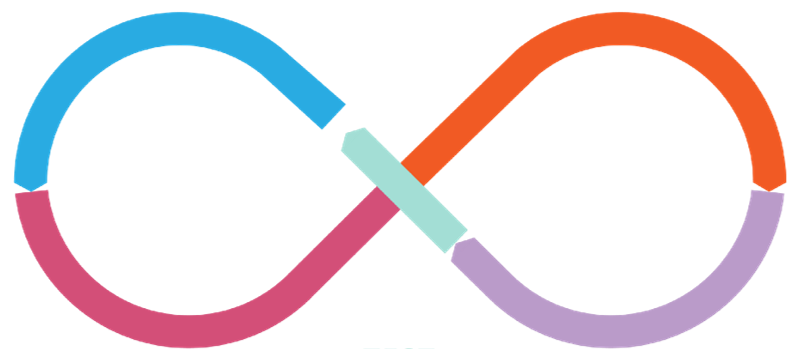
\includegraphics[width=0.65\linewidth]{process}
	\caption{Imagen inicial de la propuesta del cliente.}
	\label{fig:propuesta}
\end{figure}

También se puede poner dos subfiguras dentro de la definición de una figura (\autoref{fig:doble}), lo cual puede ser útil para hablar de dos gráficas relacionadas o algo similar. 

\begin{figure}[h!]
	\centering
	\begin{subfigure}{.45\textwidth}
		\centering
		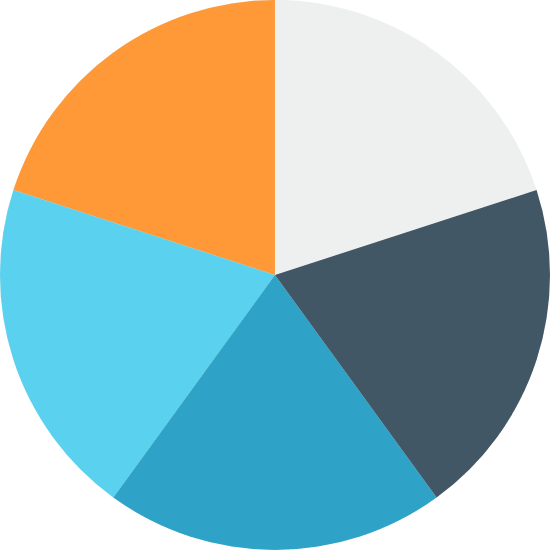
\includegraphics[width=1.7in]{pie_chart}%
		\caption{Una torta.}
		\label{fig:torta}
	\end{subfigure} 
	\hfil
	\begin{subfigure}{.45\textwidth}
		\centering
		
\includegraphics[width=1.7in]{bar_chart}%
		\caption{Unas barras}
		\label{fig:barras}
	\end{subfigure}
	\caption{Este es un caso en donde se pueden poner dos imágenes juntas, se tiene la \autoref{fig:torta} y por otro lado se tiene la \autoref{fig:barras}.}
	\label{fig:doble}
\end{figure}

\lipsum[11]

\subsubsection{Descripción del equipo}

\begin{wrapfigure}[9]{l}{0.3\linewidth}
	\vspace{-17pt}
	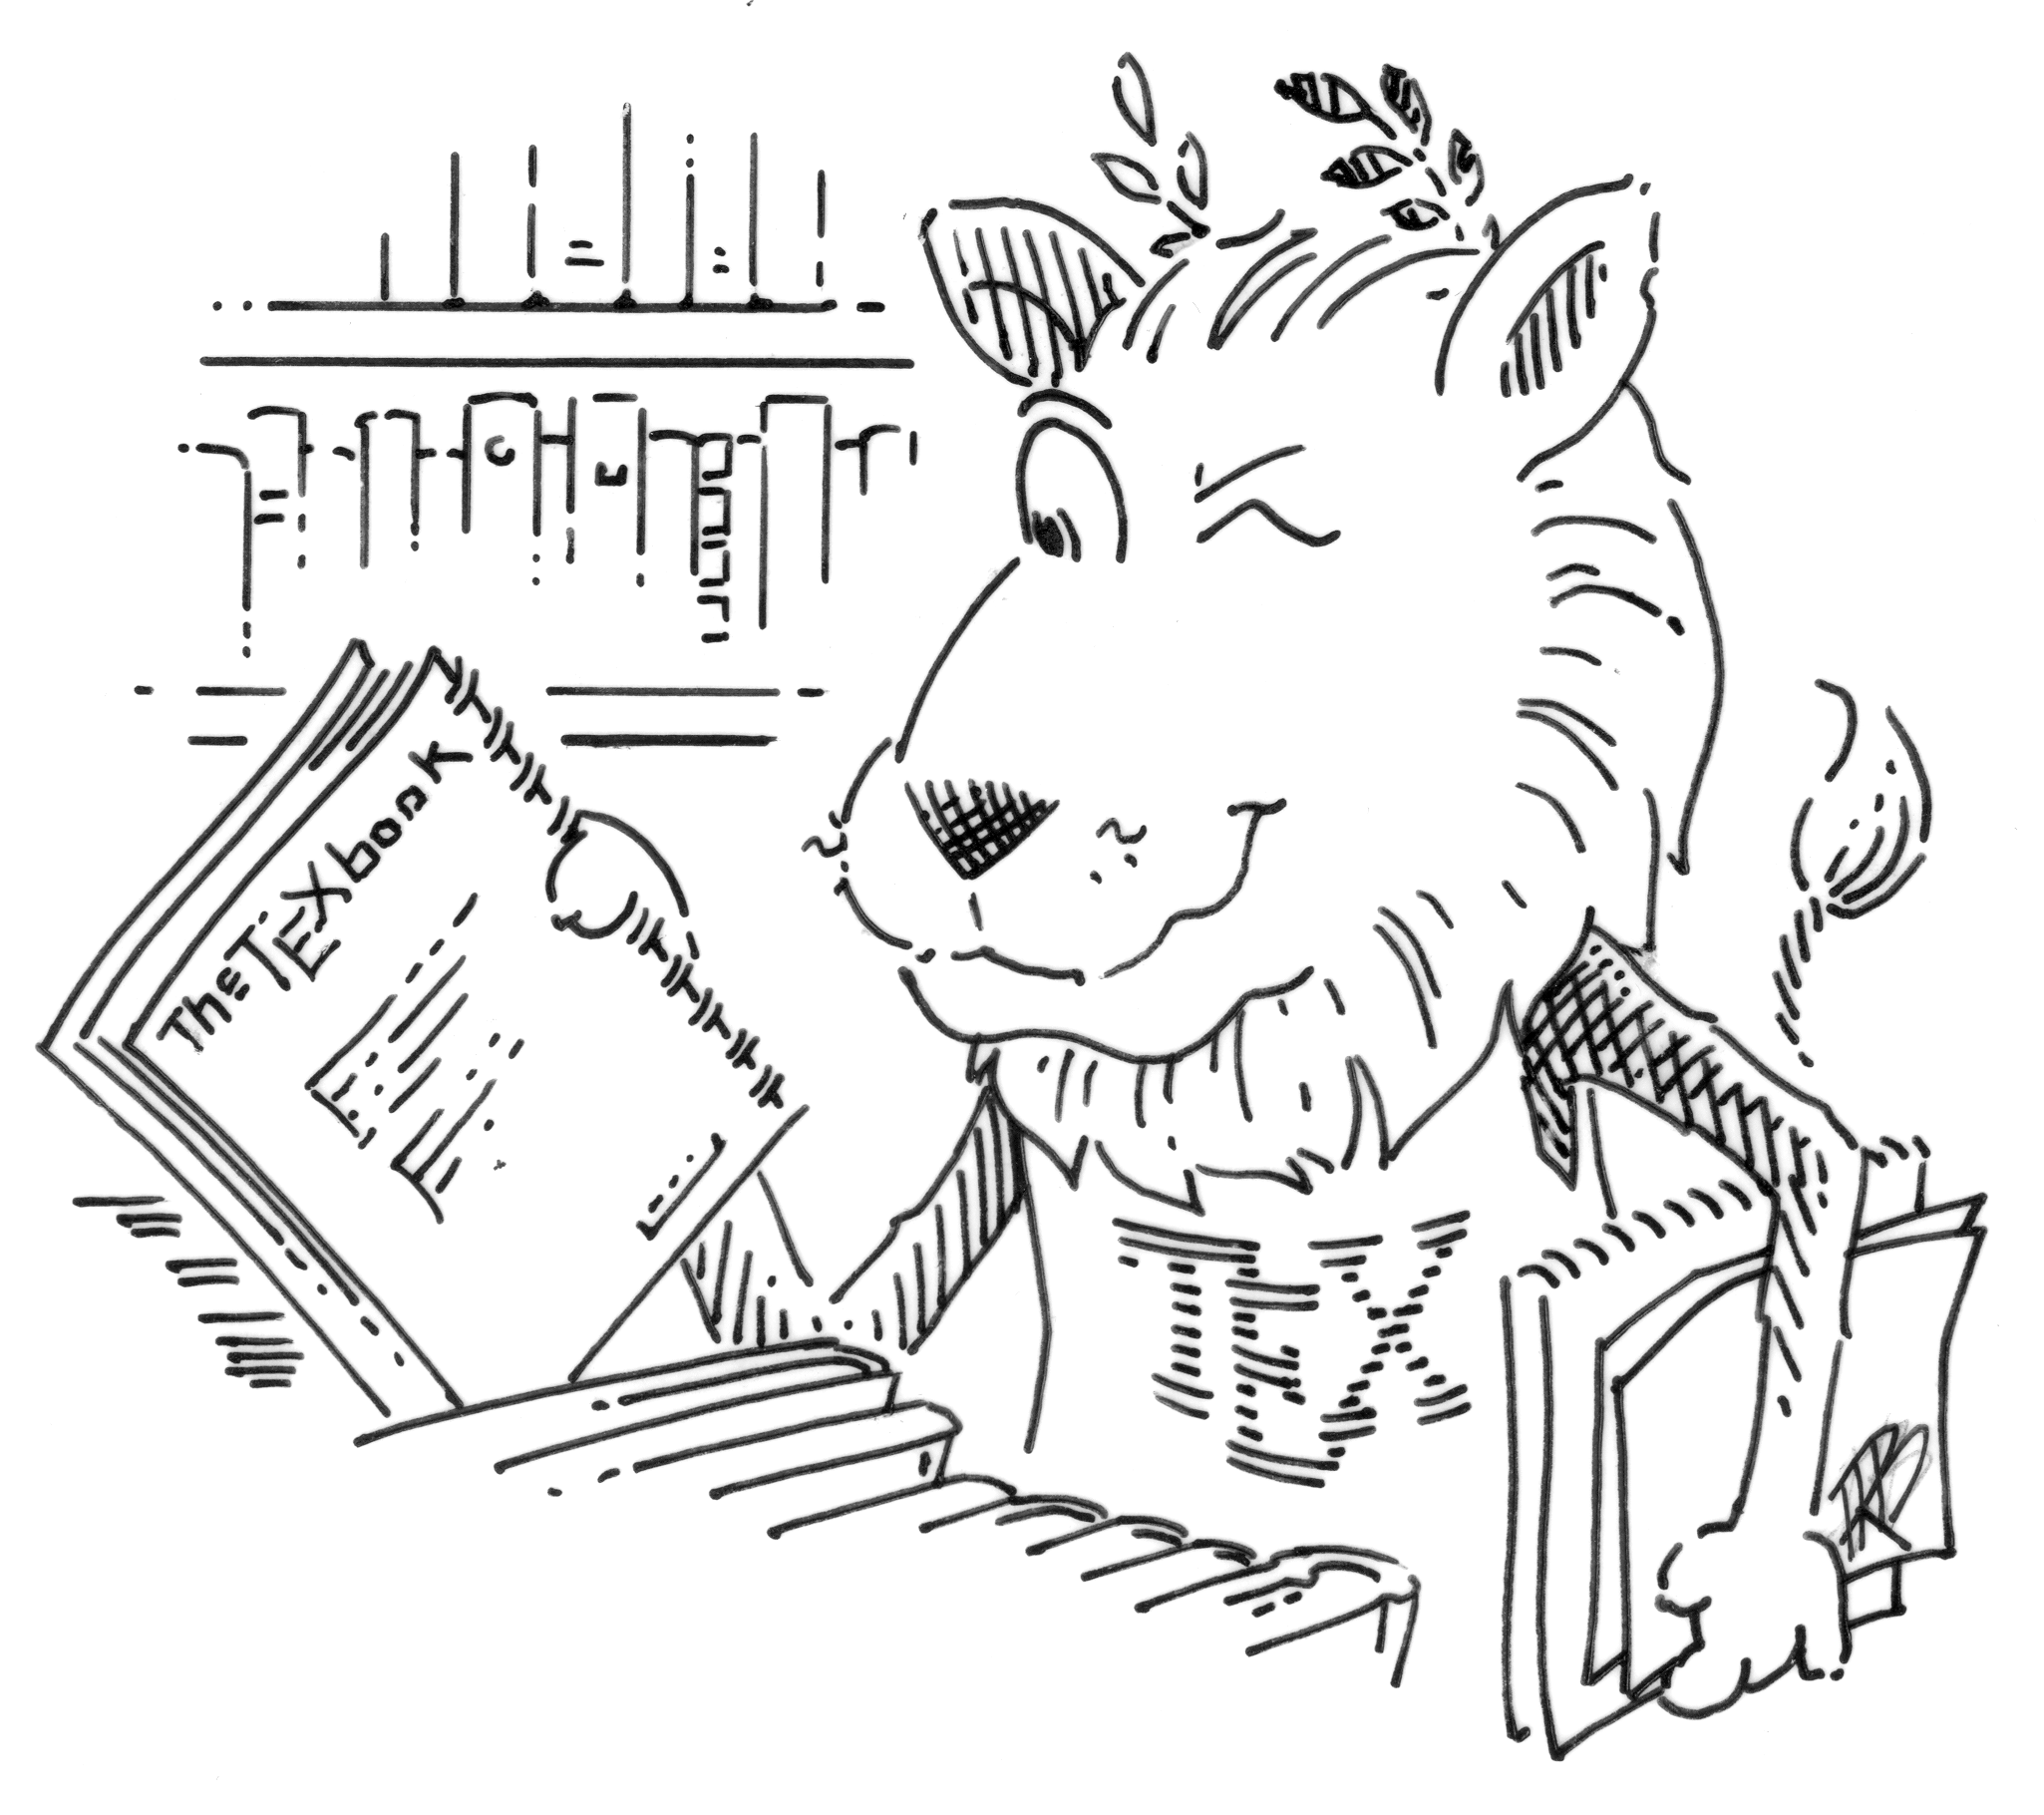
\includegraphics[width=1\linewidth]{tex_lion}
\end{wrapfigure}
\noindent {\large \textbf{\textcolor{blue}{El león de \TeX}}}\\ [5pt]
\lipsum[1]

\subsubsection{Gráfico importante}

Esto sería un gráfico importante, como el de la \autoref{fig:grafico}.

\begin{figure}[h!]
	\centering
	\begin{overpic}[width=0.6\textwidth,tics=5]{Plot} % Write ",grid" after tics to activate it. "tics" defines the grid spacing.
		\put (20,01) { 5 }
		\put (40,01) { 10 }
		\put (60,01) { 15 }
		\put (80,01) { 20 }
		\put (-2,20) { 5 }
		\put (-2,40) { 10 }
		\put (-2,60) { 15 }
		\put (63,67) {$\boxed{ f(x) = x^3 }$}
	\end{overpic}
	\caption{El camino del éxito.}
	\label{fig:grafico}
\end{figure}
\subsection{Tablas}
Lorem ipsum dolor sit amet, consectetur adipiscing elit, sed do eiusmod tempor incididunt ut labore et dolore magna aliqua. Ut enim ad minim veniam, quis nostrud exercitation ullamco laboris nisi ut aliquip ex ea commodo consequat. Duis aute irure dolor in reprehenderit in voluptate velit esse cillum dolore eu fugiat nulla pariatur.

\begin{center}
	\begin{tabular}{|l|c|c|c|}
		\hline   & 1 & 2 & 3 \\ 
		\hline A &  &  &  \\ 
		\hline B &  &  &  \\ 
		\hline 
	\end{tabular} 
\end{center}

Podemos hacer una tabla con un poco más de estilo, con ecuaciones dentro
y que se adapte el texto.
Para el Estado Límite de Servicio, los coeficientes parciales de seguridad a adoptar son los indicados en la \autoref{tab:coeficientes}.\footnote{\textcolor{grayblack}{Justo está bueno poner una nota al pie por acá.}}

\begin{table}[h]
	\centering
	\caption{Coeficientes parciales de seguridad en ELS.}
	\arrayrulecolor{grayblack}
	\rowcolors{1}{white}{gray}
	{\color{grayblack}
	\begin{tabular}{p{4cm}cc}
		\toprule
		\textbf{Tipo de acción}    & \textbf{Efecto desfavorable} & \textbf{Efecto favorable}\\
		\midrule
		Permanente & $\gamma_G=1.00$ & $\gamma_G=1.00$ \\
		Pretensado & 1.10 & 0.9 \\
		Permanente de valor no constante  & 1.00 & 1.00 \\
		Variable & 1.00 & 0.00 \\
		\bottomrule
	\end{tabular}}
	\label{tab:coeficientes}
\end{table}%

Sed ut perspiciatis unde omnis iste natus error sit voluptatem accusantium doloremque laudantium, totam rem aperiam, eaque ipsa quae ab illo inventore veritatis et quasi architecto beatae vitae dicta sunt explicabo. Nemo enim ipsam voluptatem quia voluptas sit aspernatur aut odit aut fugit, sed quia consequuntur magni dolores eos qui ratione voluptatem. 

El cronograma preliminar se presenta en la \autoref{tab:cronograma}.
	
\begin{table}[h]
	\centering
	\caption{Cronograma tentativo.}
	{\color{grayblack}
	\begin{tabular}{p{2.2em}p{14em}lllr}
		\multicolumn{1}{l}{} & \multicolumn{1}{r}{} & \multicolumn{4}{c}{\textbf{2022}} \\
		\midrule
		\textbf{Etapa} & \textbf{Productos/Entregables} & \multicolumn{1}{p{4.055em}}{\textbf{Ene-Mar}} & \multicolumn{1}{p{4.055em}}{\textbf{Abr-Jun}} & \multicolumn{1}{p{4.055em}}{\textbf{Jul-Set}} & \multicolumn{1}{p{4.055em}}{\textbf{Oct-Dic}} \\
		\midrule
		E1    & Primer documento a entregar, en .doc. &       & \cellcolor[rgb]{ .718,  .871,  .91} &       &  \\
		E2    & Segundo documento, más pesado. & \cellcolor[rgb]{ .776,  .89,  .859} &       &       &  \\
		E2    & Este tema mejor que no falte. &       & \cellcolor[rgb]{ .776,  .89,  .859} &       &  \\
		E2    & Otro tema interesante en PDF. &       &       & \cellcolor[rgb]{ .776,  .89,  .859} &  \\
		E2    & Esto es importante, también va. &       &       & \cellcolor[rgb]{ .776,  .89,  .859} &  \\
		E3    & Un documento para ver como vamos, editable. &       & \cellcolor[rgb]{ .722,  .804,  .894} &       &  \\
		E4    & Informe de evaluación hasta ahora. &       & \cellcolor[rgb]{ .722,  .804,  .894} &       &  \\
		E5    & Diseño final del sistema. &       &       &       & \cellcolor[rgb]{ .722,  .804,  .894} \\
		E6    & Recomendaciones estratégicas. &       &       &       & \cellcolor[rgb]{ .722,  .804,  .894} \\
		\bottomrule
	\end{tabular}}
	\label{tab:cronograma}
\end{table}%

\subsection{Ecuaciones}
Vamos a poner un poco de texto acá para que se note que sabemos lo que decimos. La ecuación $ E=m\cdot c^2 $. Tenemos $ f_{yk} $ o sino $ x_{a}^{2} $. También tenemos $ \frac{2}{4} $ o sino $ \dfrac{3}{4} $ o la raíz $ \sqrt{2} $.

$$ E=m\cdot c^2 $$

Como vimos en la ecuación \ref{eq:energía}. La \autoref{eq:energía} o sino la ecuación \eqref{eq:energía}.
\begin{equation} \label{eq:energía}
	E=m\cdot c^2
\end{equation}

Otra opción es una ecuación sin numerar pero dentro del entorno de ecuaciones:
\begin{equation*} \label{eq:energía2}
	E=m\cdot c^2
\end{equation*}

La suma es $ a+b $ y la resta $ a-b $. Multiplicación es $ a\cdot b$ o si no $ a \times b $. Si estoy con ángulos puedo tener $ \cos(30) $ o si no $ \sin(45) $. Una integral:
$$ \int_0^L x^2, \quad 10<15 \Rightarrow 15 \geq 10$$

Lista de ecuaciones alineadas
\begin{align}
	f(x) &= x^2+x^3			\\
	&= x^2+x^2\cdot x 
\end{align}
\begin{align*}
	f(x) &= x^2+x^3			\\
	&= x^2+x^2\cdot x 
\end{align*}
Matrices
\begin{equation*}
	A = 
	\begin{pmatrix}
		1 & 2 & 3 \\
		4 & 5 & 6 \\
		7 & 8 & 9
	\end{pmatrix}, \quad
	B = 
	\begin{bmatrix}
		1 & 2 & 3 \\
		4 & 5 & 6 \\
		7 & 8 & 9
	\end{bmatrix}, \quad
	C =
	\begin{matrix} 
		a_{11} & a_{12}  \\
		a_{21} & a_{22}  
	\end{matrix}, \quad
	D = 
	\begin{Bmatrix} 
		a_{11} & a_{12}  \\
		a_{21} & a_{22}  
	\end{Bmatrix} 
\end{equation*}
